
The refinement operators and axiom weakening operator have previously been implemented for \ALC in \cite{troquard2018repairing}. Based on this, we have extended the implementation to cover the full range of \SROIQ axioms and concepts.\footnote{The source code is available at \url{https://github.com/rolandbernard/ontologyutils}.} The concept refinement and axiom weakening operators for \SROIQ have been implemented as discussed above. Further, repair algorithms using the axiom weakening operator based also on the procedures already proposed in \cite{troquard2018repairing} and \cite{confalonieri2020towards} have been implemented. The implementation performs weakening in OWL 2 DL \cite{motik2012ontology} and is implemented in Java using the OWL API \cite{horridge2011owl,owlapi,matentzoglu2016introduction}. A plug-in for the ontology development tool Protégé has also been implemented, and will be discussed in more detail.\footnote{The Protégé plugin is available at \url{https://github.com/rolandbernard/protege-weakening}.} The plug-in allows for manually weakening axioms and executing the automatic repair algorithm.

\section{Implementing \texorpdfstring{$\SROIQ$}{SROIQ} Weakening}\label{prototype}


The implementation of the presented axiom weakening operator is based on the implementation at \cite{ontologyutils} for weakening in \ALC as discussed in \cite{troquard2018repairing}. The implementation has been significantly extended using the operators and algorithms presented in this thesis. We will now give a brief summary covering some implementation details.

The implementation has been made such that different algorithms can be used easily for repairing the ontologies. Further, for the repairs based on axiom weakening, the approaches for the selection of the reference ontology or the bad axioms are easily configurable. Additionally, the implementation contains some extra flags that can be set to modify the behaviour of the refinement and axiom weakening operators. For example, the caching explained in \cref{cache-impl} can optionally be disabled. Some other flags have been added to strictly ensure only axioms that conform to \ALC, \SROIQ, or the negation normal form of one of them are accepted and produced. Similarly, refinement of roles may optionally be disabled, used as defined in \cref{def:covers}, or can even be extended to use non-simple roles in contexts where they are allowed. In addition to the approach to weakening RIAs shown in \cref{def:weaken}, the alternative approach using a fixed preorder discussed in \cref{rbox-alternative} may be selected through a flag to the axiom weakening operator, allowing for more flexible weakening of RIAs. Note that the flags have been set up for the evaluation in \cref{evaluation} such that the weakening conforms to the definitions in \cref{weakening-sroiq}, and to accept only \SROIQ axioms.

While the implementation features the extensions to the weakening operator discussed in \cref{weakening-owl-2-dl}, to enable the evaluation of the proposed version of axiom weakening operating only on \SROIQ concepts and axioms, the ontologies had to be normalized. To achieve this, axioms and concepts had to be modified. For TBox axioms, the OWL API is already able to do most of the work by providing a method that converts axioms into one or more GCIs. For ABox axioms, the only transformation that had to be done is converting $n$-ary same individual and different individuals axioms to $\frac{n (n - 1)}{2}$ different binary equalities and inequalities. In the case of same individual axioms, there is also a flag that will cause the normalization to generate only $n - 1$ equalities, such that one of the individuals is asserted to be equal to all the others. The same mechanisms have been implemented for RBox axioms asserting equivalence or disjointness between roles. The rest of the RBox axioms have been transformed into RIAs and GCIs. There are only two kinds of concepts that had to be specially handled. The exact cardinality constraint is transformed into a conjunction between an at-least and an at-most constraint. The has-value constraint is transformed by using an existential quantification and nominal concept. Further details on the implemented translation can be found in \cref{owl-to-sroiq}.

\begin{algorithm}[ht]
  \begin{algorithmic}
    \State $\Omcfull \gets \Omc$
    \State $\Omcref \gets \textsc{FindConsistentSubset}(\Omc)$
    \While{$\Omc$ is inconsistent}
      \State $\phi_\textnormal{bad} \gets \textsc{FindBadAxiom}(\Omc)$
      \State $\phi_\textnormal{weaker} \gets \textsc{SelectWeakerAxiom}(g_{\Omcref,\Omcfull}(\phi_\textnormal{bad}))$
      \State $\Omc \gets (\Omc \setminus \{\phi_\textnormal{bad}\}) \cup \{\phi_\textnormal{weaker}\}$
    \EndWhile
    \State Return $\Omc$
  \end{algorithmic}
  \caption{$\textsc{RepairOntologyWeaken}(\Omc)$}
  \label{algo:repair-weaken}
\end{algorithm}

The automatic repair algorithm using axiom weakening has been implemented as depicted in \cref{algo:repair-weaken}. It repeatedly selects ``bad axioms'' and replaces them with weaker axioms generated by means of the axiom weakening operator defined in \cref{def:weaken}. This is repeated until the ontology becomes consistent. In the implementation used for the evaluation in this thesis, the reference ontology has been selected by randomly sampling a maximal consistent subset. The prototype does, however, also include multiple alternative implementations of $\textsc{FindConsistentSubset}$. One is to choose as reference ontology the intersection of some (or all) maximal consistent subsets, while another is to select one of the largest (in terms of the number of axioms) maximal consistent subsets. Note that the implementation will consider ontologies as the union of some static axioms $\Omc_s$ and some refutable axioms $\Omc_r$, as defined in \cref{basic-definitions}. This has been taken into account for the computation of maximal consistent subsets in $\textsc{FindBadAxiom}$. One reason for the split into static and refutable axioms is to keep non-logical axioms, like declarations and annotations, in every tested ontology. Especially declaration axioms must be kept, because OWL 2 DL mandates that every signature element must be declared, and otherwise some reasoners will produce incorrect results or throw errors.

The procedure $\textsc{FindBadAxiom}$ may also be implemented in several different ways. For the evaluation, we consider an implementation that randomly samples some (or all) minimal inconsistent subsets of axioms $J_1, J_2, \dots, J_k \subseteq \Omc$ and selects as the bad axiom the one occurring most frequently. The implementation contains also some other implementations of $\textsc{FindBadAxiom}$, e.g., selecting a random axiom, selecting the axiom that appears in the least maximal consistent subsets, or selecting an axiom that does not appear in the largest (by axiom count) maximal consistent subset. The implementation of $\textsc{FindBadAxiom}$ is such that it will only ever return axioms $\alpha \in \Omc_r$. To do this, minimal subsets $J$ of $\Omc_r$ such that $J \cup \Omc_s$ is inconsistent are sampled. With this feature, a variation of the repair using axiom weakening has been implemented, in which the axioms of the reference ontology $\Omcref$ are not weakened during the repair. This has been done by, after computing $\Omcref$, setting $\Omc_s \gets \Omc_s \cup \Omcref$ and $\Omc_r \gets \Omc_r \setminus \Omcref$. This variation has been evaluated in \cref{eval-quality}.

\subsection{Performance}\label{performance-impl}

The prototype implementation uses the OWL API \cite{horridge2011owl,owlapi} to represent axioms in memory and interface with off-the-shelf reasoners. The reasoners FaCT++, JFact, HermiT, and Openllet have been used in the prototype. Creating a new reasoner instance for each time an entailment is checked or consistency must be tested is however inefficient. One reason for this is that instantiating a reasoner is relatively expensive. Further, all the mentioned reasoners are, to some degree, able to keep some information computed for previous queries and exploit it to speed up subsequent ones. For these reasons, it is desirable to reuse reasoners as much as possible. To facilitate this, a class \inlinecode{Ontology} has been created that contains a set of axioms (split into static $\Omc_s$ and refutable $\Omc_r$) as well as a reference to a set of already initialized reasoners. This class contains the methods for checking consistency and entailment, implementing them by taking one of the initialized reasoners, updating the reasoner's internal state by adding and removing axioms to reflect the state of the ontologies axioms, and then calling the reasoners axioms. Only if no reasoner is available, will a new one be created and initialized. One thing this setup allows for is the creation of multiple ontologies that point to the same set of reasoners. To achieve this, it is recorded which ontologies use the reasoners, and if they are no longer needed, they can be disposed of to free up global resources.

To improve performance, particularly for running the test cases, running work in parallel has been considered. One problem with this approach is that all reasoners are linked to a global \inlinecode{OWLOntologyManager} object. There is a concurrent version of this object, but not all reasoners are implemented in a way to make concurrent access to this object possible. The FaCT++ reasoner \cite{factpp} had a significantly severe problem, where it would listen to and apply all changes made to any ontology in the ontology manager. Since this manager can, however, contain multiple ontologies, this lead to wrong reasoning results. These issues have been resolved in the slightly modified version of the FaCT++ reasoner used for this thesis.\footnote{The version of FaCT++ used for this thesis is available at \url{https://github.com/rolandbernard/factplusplus}} This version had some further modifications, like fixing an issue with the handling of annotated axioms and adding automatic loading of native dependencies, something for which previously an environment variable had to be set pointing at the dynamic library. After these changes, and some additional modifications in the prototype code, the tests can now be run concurrently. Further, the prototype contains some experiments that use multiple threads, sharing the same axiom weakening operator and cache, to compute multiple weakenings in parallel.

\subsection{Computing Minimal Subsets}\label{minimal-set-impl}

For some operations, maximal consistent subsets and minimal inconsistent subsets of an ontology $\Omc$ must be computed. As has been observed in \cite{marques2013minimal} for the case of propositional logic, these problems can both be reduced to the problem of finding a minimal subset over some monotone predicate. This is also true for DLs. A predicate $p$ is monotone if for every two sets $A$ and $B$ where $A \subseteq B$, $p(A) \implies p(B)$. Given a monotone predicate $p$ and a set $A$, the problem is to find a subset $J$ of $A$ such that $p(J)$ and for all subsets $J'$ of $J$, $p(J')$ does not hold. The problem of finding a minimal inconsistent subset can trivially be reduced to this problem by setting $A = \Omc_r$ and $p_\textnormal{MIS}(A) \iff \Omc_s \cup A \models \top \sqsubseteq \bot$. Instead of finding the maximal consistent subset, we can find the minimal subset such that removing it from the full ontology results in a consistent ontology. That is, we solve the minimal subset problem over the set $A = \Omc_r$ using the predicate $p_\textnormal{MCS}(A) \iff \Omc_s \cup \Omc_r \setminus A \not\models \top \sqsubseteq \bot$. Removing this minimal subset will yield a maximal consistent subset since adding any other axiom is equivalent to removing fewer axioms, and since the set is minimal, there is no way to remove fewer axioms and still satisfy the predicate.

\begin{algorithm}[ht]
  \begin{algorithmic}
    \State $A' \gets A$
    \For{$a \in A$}
      \If{$p(A' \setminus \{ a \})$}
        \State $A' \gets A' \setminus \{ a \}$
      \EndIf
    \EndFor
    \State Return $A'$
  \end{algorithmic}
  \caption{$\textsc{SimpleFindMinimalSubset}(A, p)$}
  \label{algo:find-minimal-subset-simple}
\end{algorithm}

One simple way to compute a single minimal subset is by starting with the complete set. Then one goes through all the elements and tries to remove them. If after removal the predicate still holds, the element is removed, otherwise, it is kept. This algorithm is listed in \cref{algo:find-minimal-subset-simple}. After having tested and possibly removed all elements, the remaining elements form a minimal subset. To see this, assume we end up with a set $A'$ and there exists an element $a \in A'$ for which $p(A' \setminus \{ a \})$ is true. Since all elements in $A$ have already been tested once, $p(A'' \setminus \{ a \})$ was false for some set $A'' \supseteq A'$. However, this means $A' \setminus \{ a \} \subseteq A'' \setminus \{ a \}$ and since $p$ is monotone and $p(A' \setminus \{ a \})$ is true, $p(A'' \setminus \{ a \})$ must also be true. This is a contradiction since if $p(A'' \setminus \{ a \})$ had been true we would have removed $a$ from the set.

\begin{algorithm}[ht]
  \begin{algorithmic}
    \State Choose some permutation $a_1, a_2, \cdots, a_n$ of $A$
    \State $A' \gets \emptyset$, \enspace $i \gets 1$, \enspace $s \gets 1$
    \While{$i \leq n$}
      \If{$p(A' \cup \{ a_{i + s}, a_{i + s + 1}, \cdots, a_n \})$}
        \State $i \gets i + s$, \enspace $s \gets 2 s$
      \Else
        \State $l \gets i$, \enspace $r \gets i + s - 1$
        \While{$l < r$}
          \State $m \gets \lceil \frac{l + r}{2} \rceil$
          \If{$p(A' \cup \{ a_m, a_{m + 1}, \cdots, a_n \})$}
            \State $l \gets m$
          \Else
            \State $r \gets m - 1$
          \EndIf
        \EndWhile
        \State $A' \gets A' \cup \{ a_l \}$, \enspace $i \gets l + 1$, \enspace $s \gets 1$
      \EndIf
    \EndWhile
    \State Return $A'$
  \end{algorithmic}
  \caption{$\textsc{FindMinimalSubset}(A, p)$}
  \label{algo:find-minimal-subset}
\end{algorithm}

This same idea can be made somewhat more efficient in cases where the minimal subsets are only relatively small compared to the complete set. This is often the case for finding minimal inconsistent subsets or minimal correction subsets. For this, the progression-based algorithm presented in \cite{marques2013minimal} has been implemented. The algorithm works by trying to remove more than one element at a time, and if that fails, binary search is used to locate the first element which must be included in the minimal set.
To compute multiple (but not necessarily all) minimal sets, the \textsc{MergeXplain} algorithm proposed in \cite{shchekotykhin2015mergexplain} has also been implemented, but was not used during the evaluation.

\begin{algorithm}[ht]
  \begin{algorithmic}
    \State Globals \enspace $B \gets \emptyset$, \enspace $M \gets \emptyset$ \quad (initialized once)
    \If{$\forall b \in B : A \not\subseteq b $}
      \If{$\exists m' \in M : m' \subseteq A$}
        \State $m \gets m'$
      \ElsIf{$p(A)$}
        \State $m \gets \textsc{FindMinimalSubset}(A, p)$
        \State $M \gets M \cup \{ m \}$
      \Else
        \State $m \gets \emptyset$
      \EndIf
      \For{$a \in m$}
        \State $\textsc{FindAllMinimalSubsets}(A \setminus \{ a \}, p)$
      \EndFor
      \State $B \gets B \cup \{ A \}$
    \EndIf
    \State $M$ contains the set of all minimal subsets after the DFS terminates.
  \end{algorithmic}
  \caption{$\textsc{FindAllMinimalSubsets}(A, p)$}
  \label{algo:find-minimal-subsets}
\end{algorithm}

Similarly, an algorithm for finding all minimal subsets has been implemented as shown in \cref{algo:find-minimal-subsets}. The algorithm is based on the hitting-set-tree algorithm \cite{reiter1987theory} and is based on the approach proposed in \cite{kalyanpur2007finding}. The idea is to use a depth-first search on the hitting-set-tree. In this tree, every node is labelled with a minimal subset, and every edge is labelled with an element of the minimal subset in the parent. The elements labelling the edges on the path from the root to a node are removed from the complete set before finding a minimal subset with which to label the node. To find the minimal subset, the procedure in $\textsc{FindMinimalSubset}$ can be used. If no such minimal subset exists, then the search in the current branch is finished, because no subset will contain any minimal subsets either. Minimal subsets may be reused to label multiple nodes, making the search more efficient. Additionally, early path pruning can be performed to avoid testing the same subsets multiple times.

\subsection{Caching for Faster Repairs}\label{cache-impl}

The implementation will spend most of its time during repairs calling the reasoner to compute consistency and entailment queries. In order to reduce the number of calls that must be made and to accelerate the computation of upward and downward cover sets, some caching has been added. Since upward and downward covers must potentially be computed many times for a single application of the refinement or axiom weakening operators, it is an obvious point to optimize. Further, since the reference ontology and full ontology have been chosen to remain fixed for the duration of the repair, the upward and downward cover functions remain constant. When following directly the definition of cover sets presented in \cref{def:covers}, one will compute numerous subsumptions, many of which will be the same across multiple cover computations. This is therefore the aspect that caching has been applied to. The reasoners used in the implementation already have the ability to partially reuse previous results when computing queries. We, therefore, made sure to reuse the same reasoner instances wherever possible, to exploit this feature.

Rather than rely solely on the internal reuse of the reasoner or apply only a simple cache, however, we found it worthwhile to create a cache for subsumption, in which extra information is also inferred from the transitivity of subsumption after each query to the reasoner. This is in effect similar to the technique presented in \cite{shearer2009exploiting} for creating taxonomies, but applied also to complex concepts. Additionally, some basic rules were added to compute subsumption involving conjunctions and disjunctions, by using the results computed for the conjuncts or disjuncts of the expression. Another difference, with respect to the computation of taxonomies, is that subsumptions are computed only when requested. While pre-computing the complete relation over the subconcepts would allow for ordering of the reasoner queries to maximize information gain, like one may do when computing taxonomies, this turned out to be disadvantageous, since in general, a single repair will not require all results. 

\begin{algorithm}[ht]
  \begin{algorithmic}
    \State Globals \enspace $S \gets \emptyset$, \enspace $K \gets \emptyset$, \enspace $P \gets \emptyset$ \quad (initialized once)
    \For{$X \in \{ C, D \}$ where $X \not\in S$}
      \State $S \gets S \cup \{ X \}$
      \State $K \gets K \cup \{ \langle X, X \rangle \}$
      \State $P \gets P \cup ( S \times \{ X \} ) \cup ( \{ X \} \times S )$
    \EndFor
    \If{$\langle C, D \rangle \in K$}
      \State $R \gets \mathit{True}$
    \ElsIf{$\langle C, D \rangle \not\in P$}
      \State $R \gets \mathit{False}$
    \Else
      \State $R \gets \textsc{TestSubsumtion}(C, D)$
      \If{$R$}
        \State $K \gets K \cup \{ \langle C', D' \rangle \mid \langle C', C \rangle \in K \text{ and } \langle D, D' \rangle \in K \}$
        \State $P \gets P \setminus \{ \langle D, D' \rangle \mid \langle D', C' \rangle \in K \text{ and } \langle C, C' \rangle \not\in P \}$
        \State $P \gets P \setminus \{ \langle C', C \rangle \mid \langle D', C' \rangle \in K \text{ and } \langle D', D \rangle \not\in P \}$
      \Else
        \State $P \gets P \setminus \{ \langle C', D' \rangle \mid \langle C, C' \rangle \in K \text{ and } \langle D', D \rangle \in K \}$
      \EndIf
    \EndIf
    \State Return $R$
  \end{algorithmic}
  \caption{$\textsc{CachedTestSubsumtion}(C, D)$}
  \label{algo:cached-subs}
\end{algorithm}

It follows a brief description of the algorithm used for caching subsumptions listed in \cref{algo:cached-subs}. We keep three global variables, the set of all elements that have already been encountered at least once $S$, the set of know tuples $K$, and the set of possible tuples $P$. When querying a subsumption, it is first ensured that if one or both of the elements has not yet been seen before, the appropriate tuples are inserted into $K$ and $P$. Then it is checked whether the result can be determined using the known information, and if not, the procedure $\textsc{TestSubsumtion}$ is used to compute the correct result. For every new negative result, the possible tuples are reduced and for every positive result, known tuples are added, and possible tuples may also be removed. The algorithm is based on the two implications
\begin{align*}
  C \sqsubseteq_\Omc D \text{ and } D \sqsubseteq_\Omc E &\implies C \sqsubseteq_\Omc E \enspace,\text{ and} \\
  C \not\sqsubseteq_\Omc D \text{ and } C \sqsubseteq_\Omc E \text{ and } F \sqsubseteq_\Omc D &\implies E \not\sqsubseteq_\Omc F \enspace.
\end{align*}
The first implication follows trivially from the fact that subsumption between concepts or roles is transitive. The second also follows from transitivity. It can be observed that, if $C \sqsubseteq_\Omc E$ and $F \sqsubseteq_\Omc D$, if $E \sqsubseteq_\Omc F$ were to hold, then $C \sqsubseteq_\Omc D$ would also have to hold by transitivity. Separate instances of $S$, $K$ and $P$ are used for the computation of concept and role subsumptions.

For actually computing subsumptions between roles, $\textsc{TestSubsumtion}$ is a simple call to the reasoner. However, for computing subsumption between concepts, one further step is used. It is applied immediately before possibly calling the reasoner. If any of the following rules can be computed using only the information in $S$, $K$, and $P$, the reasoner is not called, and the result returned from $\textsc{TestSubsumtion}$. Otherwise, the reasoner is used as usual to compute the subsumption.
\begin{align*}
  C_i \not\sqsubseteq_\Omc D \text{ for some } i \in \{ 1, \dots, n \} &\implies C_1 \sqcup \cdots \sqcup C_n \not\sqsubseteq_\Omc D \\
  C_i \sqsubseteq_\Omc D \text{ for all } i \in \{ 1, \dots, n \} &\implies C_1 \sqcup \cdots \sqcup C_n \sqsubseteq_\Omc D \\
  C \not\sqsubseteq_\Omc D_i \text{ for some } i \in \{ 1, \dots, n \} &\implies C \not\sqsubseteq_\Omc D_1 \sqcap \cdots \sqcap D_n \\
  C \sqsubseteq_\Omc D_i \text{ for all } i \in \{ 1, \dots, n \} &\implies C \sqsubseteq_\Omc D_1 \sqcap \cdots \sqcap D_n \\
  C_i \sqsubseteq_\Omc D \text{ for some } i \in \{ 1, \dots, n \} &\implies C_1 \sqcap \dots \sqcap C_n \sqsubseteq_\Omc D \\
  C \sqsubseteq_\Omc D_i \text{ for some } i \in \{ 1, \dots, n \} &\implies C \sqsubseteq_\Omc D_1 \sqcup \cdots \sqcup D_n \\
\end{align*}

\subsection{Finding Best Repairs}\label{best-repair-impl}

The implementation contains also some approaches for finding the ``best repair'' based on some quality function given to the algorithm. None of these algorithms were however evaluated since they are significantly slower than the others, needing to compute not only multiple repairs but also the quality estimation for each of them. The simplest algorithm implemented for this purpose simply computes some (or all) maximal consistent subsets and selects the one that performs the based on the given function. Another is to compute multiple repairs using axiom weakening, following the algorithm in \cref{algo:repair-weaken}, and select the one that has the highest quality based on the given function. A more sophisticated approach that was also realized is to apply a Monte-Carlo search \cite{coulom2006efficient} based algorithm to explore the tree formed by weakening. In this case, both the possible choices of bad axioms and the selection of the weakening are explored using search.



\section{Axiom Weakening in Protégé}\label{protege}


The Protégé plugin reuses much of the code written for the above-mentioned implementation. For the implementation, the information in the developer documentation \cite{protege5devdocs} has been consulted. Additionally, the implementation of other plugins \cite{ontodebug,protegepluginexamples} has been used as a basis for the plugin. It would have been desirable to share the same codebase between the two implementations, but some choices made for the prototype implementation were incompatible with it's the later use in the plugin. While Protégé is also using the OWL API, it is not using the latest version. Since for the implementation discussed in \cref{prototype} the latest OWL API version was used, and the two are not compatible, some changes had to be made. Further, the prototype has as dependencies the different OWL reasoners, this is a problem because those might not be included in Protégé, and bundling them with the plugin might cause conflicts if they are actually in Protégé already. For this reason, the implementation has been adapted to use the reasoner that is currently selected by the user in Protégé. Additionally, but less impactful, is also that Protégé uses an older version of Java than what has been used for the prototype implementation build for the evaluation. Three different ways to interact with the axiom weakening methods have been implemented in this plugin, we will show now each of them in turn.

\begin{figure}[ht]
  \centering
  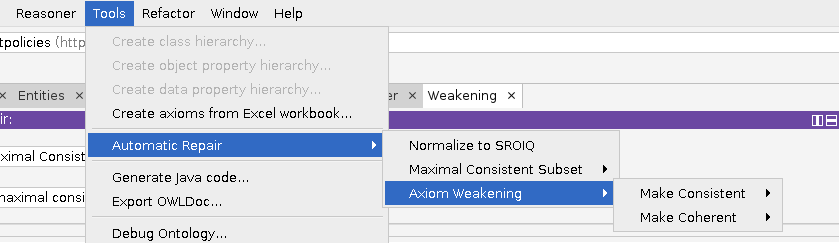
\includegraphics[width=\textwidth]{resources/protege-menu.png}
  \caption{Screenshot of the Protégé menu items added by the plugin.}
  \label{fig:protege-menu}
\end{figure}

In order to quickly apply the normalization, or automatic repair algorithms, some menu items have been added by the plugin under ``Tools''. The first menu item, ``Normalize to SROIQ'', allows the quick application of the normalization, described in \cref{owl-to-sroiq}. Then there are two different repair algorithms for which menu entries have been added. The first, used by ``Maximal Consistent Subset'' selects as the repair a randomly selected maximal consistent subset. The second, used with ``Axiom Weakening'', is based on the algorithm listed in \cref{algo:repair-weaken}. For each of these two algorithms, the user may choose between making the ontology only consistent, or making it also coherent. The repair for making the ontology coherent works analogously to the one for making the ontology consistent, except that the tests for consistency of the ontology are replaced with tests for coherence.

\begin{figure}[ht]
  \centering
  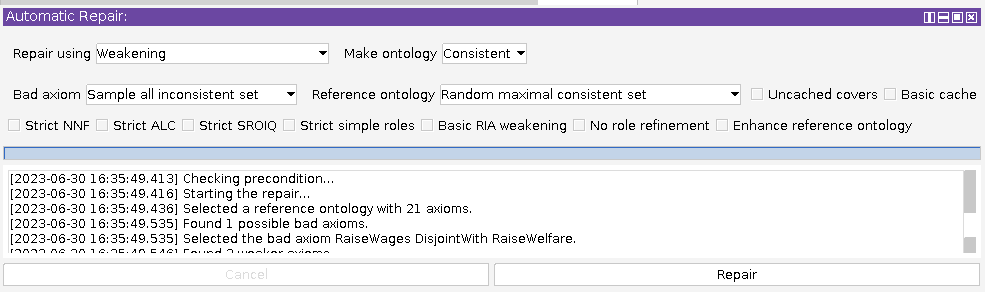
\includegraphics[width=\textwidth]{resources/protege-repair.png}
  \caption{Screenshot of the Protégé view added by the plugin, allowing for configuring and applying repairs algorithms.}
  \label{fig:protege-repair}
\end{figure}

The second method of interacting with the proposed axiom weakening repair algorithms is through a more detailed view added by the plugin. The user can select both the algorithm, e.g., by removal, using a maximally consistent set, using axiom weakening, etc., and the goal of the repair, i.e., consistency or coherence. Further, for some repair methods, options are made available. For the repair by weakening, all the flags and variations discussed in \cref{prototype} can be configured, as can be seen in \cref{fig:protege-repair}. Below the section for configuring the repair algorithm, a progress indicator and log have been placed. For long-running repairs, this is a valuable addition so that the user can see that the repair is still running. Another important feature that has been added specifically for the plugin is the ability to interrupt the repairs. To facilitate this functionality, the repair is started in a separate thread, and before every reasoner call, the implementation checks whether the thread has been interrupted, and if it has the repair is terminated by throwing an exception.

\begin{figure}[ht]
  \centering
  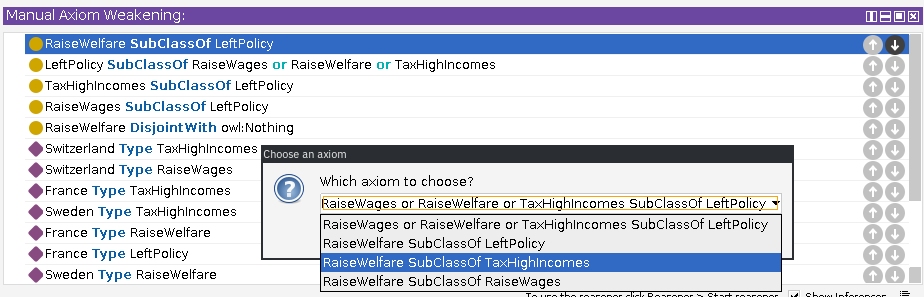
\includegraphics[width=\textwidth]{resources/protege-manual.png}
  \caption{Screenshot of the Protégé view added by the plugin, allowing for manually selecting axioms and weakening them.}
  \label{fig:protege-manual}
\end{figure}

Lastly, a view has been added that allows users to manually select how they want to weaken axioms. The view, depicted in \cref{fig:protege-manual}, shows a list of all axioms. The axioms are sorted by how frequently they appear in some minimal inconsistent subsets that are randomly sampled. The axioms that appear the most often are shown first, such that the axioms that are shown at the top of the list are the ones that would be selected by the automatic repair algorithm. The two buttons next to the axioms with the upward and downward arrow can then be used to, respectively, show weaker or stronger axioms. The user may choose one of these refined axiom to replace the original axiom.


